\documentclass[11pt,letterpaper]{article}
\usepackage[margin=1in]{geometry}
\usepackage{graphicx}
\usepackage{hyperref}
\usepackage{booktabs}
\usepackage{enumitem}
\usepackage{titlesec}
\usepackage{parskip}
\usepackage{xcolor}
\usepackage{fancyhdr}
\usepackage{caption}

\hypersetup{colorlinks=true, linkcolor=teal, urlcolor=teal, citecolor=teal}

\pagestyle{fancy}
\fancyhf{}
\rhead{CampusPark -- Final Project Report}
\lhead{INFO 5100}
\cfoot{\thepage}

\title{\textbf{CampusPark}\\[4pt]
\large Smart Campus Parking Reservation System\\[2pt]
\normalsize Final Project Report -- Phase II}
\author{Guanya Song}
\date{April 2026}

\begin{document}
\maketitle
\thispagestyle{fancy}

% ─────────────────────────────────────────────
\section{Project Overview}

CampusPark is a web application for reserving campus parking spots around the
Seattle area. Students and visitors can search available lots, book a spot in
advance, check in at the gate with a 6-digit ticket code, and check out with
automatic fee calculation. Administrators get a dashboard showing occupancy,
revenue, and user activity over time.

The motivation came from how hard it is to find parking on campus when you arrive
without knowing which lots are full. Most systems only show a static map. This
project tries to fix that by showing live availability and helping users pick a
lot based on where they are coming from.

The three main parts of the system are:

\begin{enumerate}[leftmargin=1.4em]
  \item \textbf{Live availability} -- spot counters update every time a reservation
        is created, checked in, or cancelled. A background job also simulates
        realistic occupancy changes every 15 minutes.
  \item \textbf{Route-based recommendation} -- the user enters a departure address
        or ZIP code, the server geocodes it, and then scores each parking lot by
        distance, price, and availability to suggest the best option.
  \item \textbf{Reservation lifecycle} -- a booking starts as PENDING,
        transitions to ACTIVE after ticket check-in, and closes as COMPLETED
        once the user checks out. Unclaimed PENDING reservations expire after
        5 minutes so the spot becomes available again.
\end{enumerate}

% ─────────────────────────────────────────────
\section{System Architecture}

\subsection{UML Component Diagram}

Figure~\ref{fig:uml} is the component diagram from Assignment 5.
It shows the four main layers: the browser client, the Node.js backend,
the Prisma ORM, and PostgreSQL.

\begin{figure}[h]
  \centering
  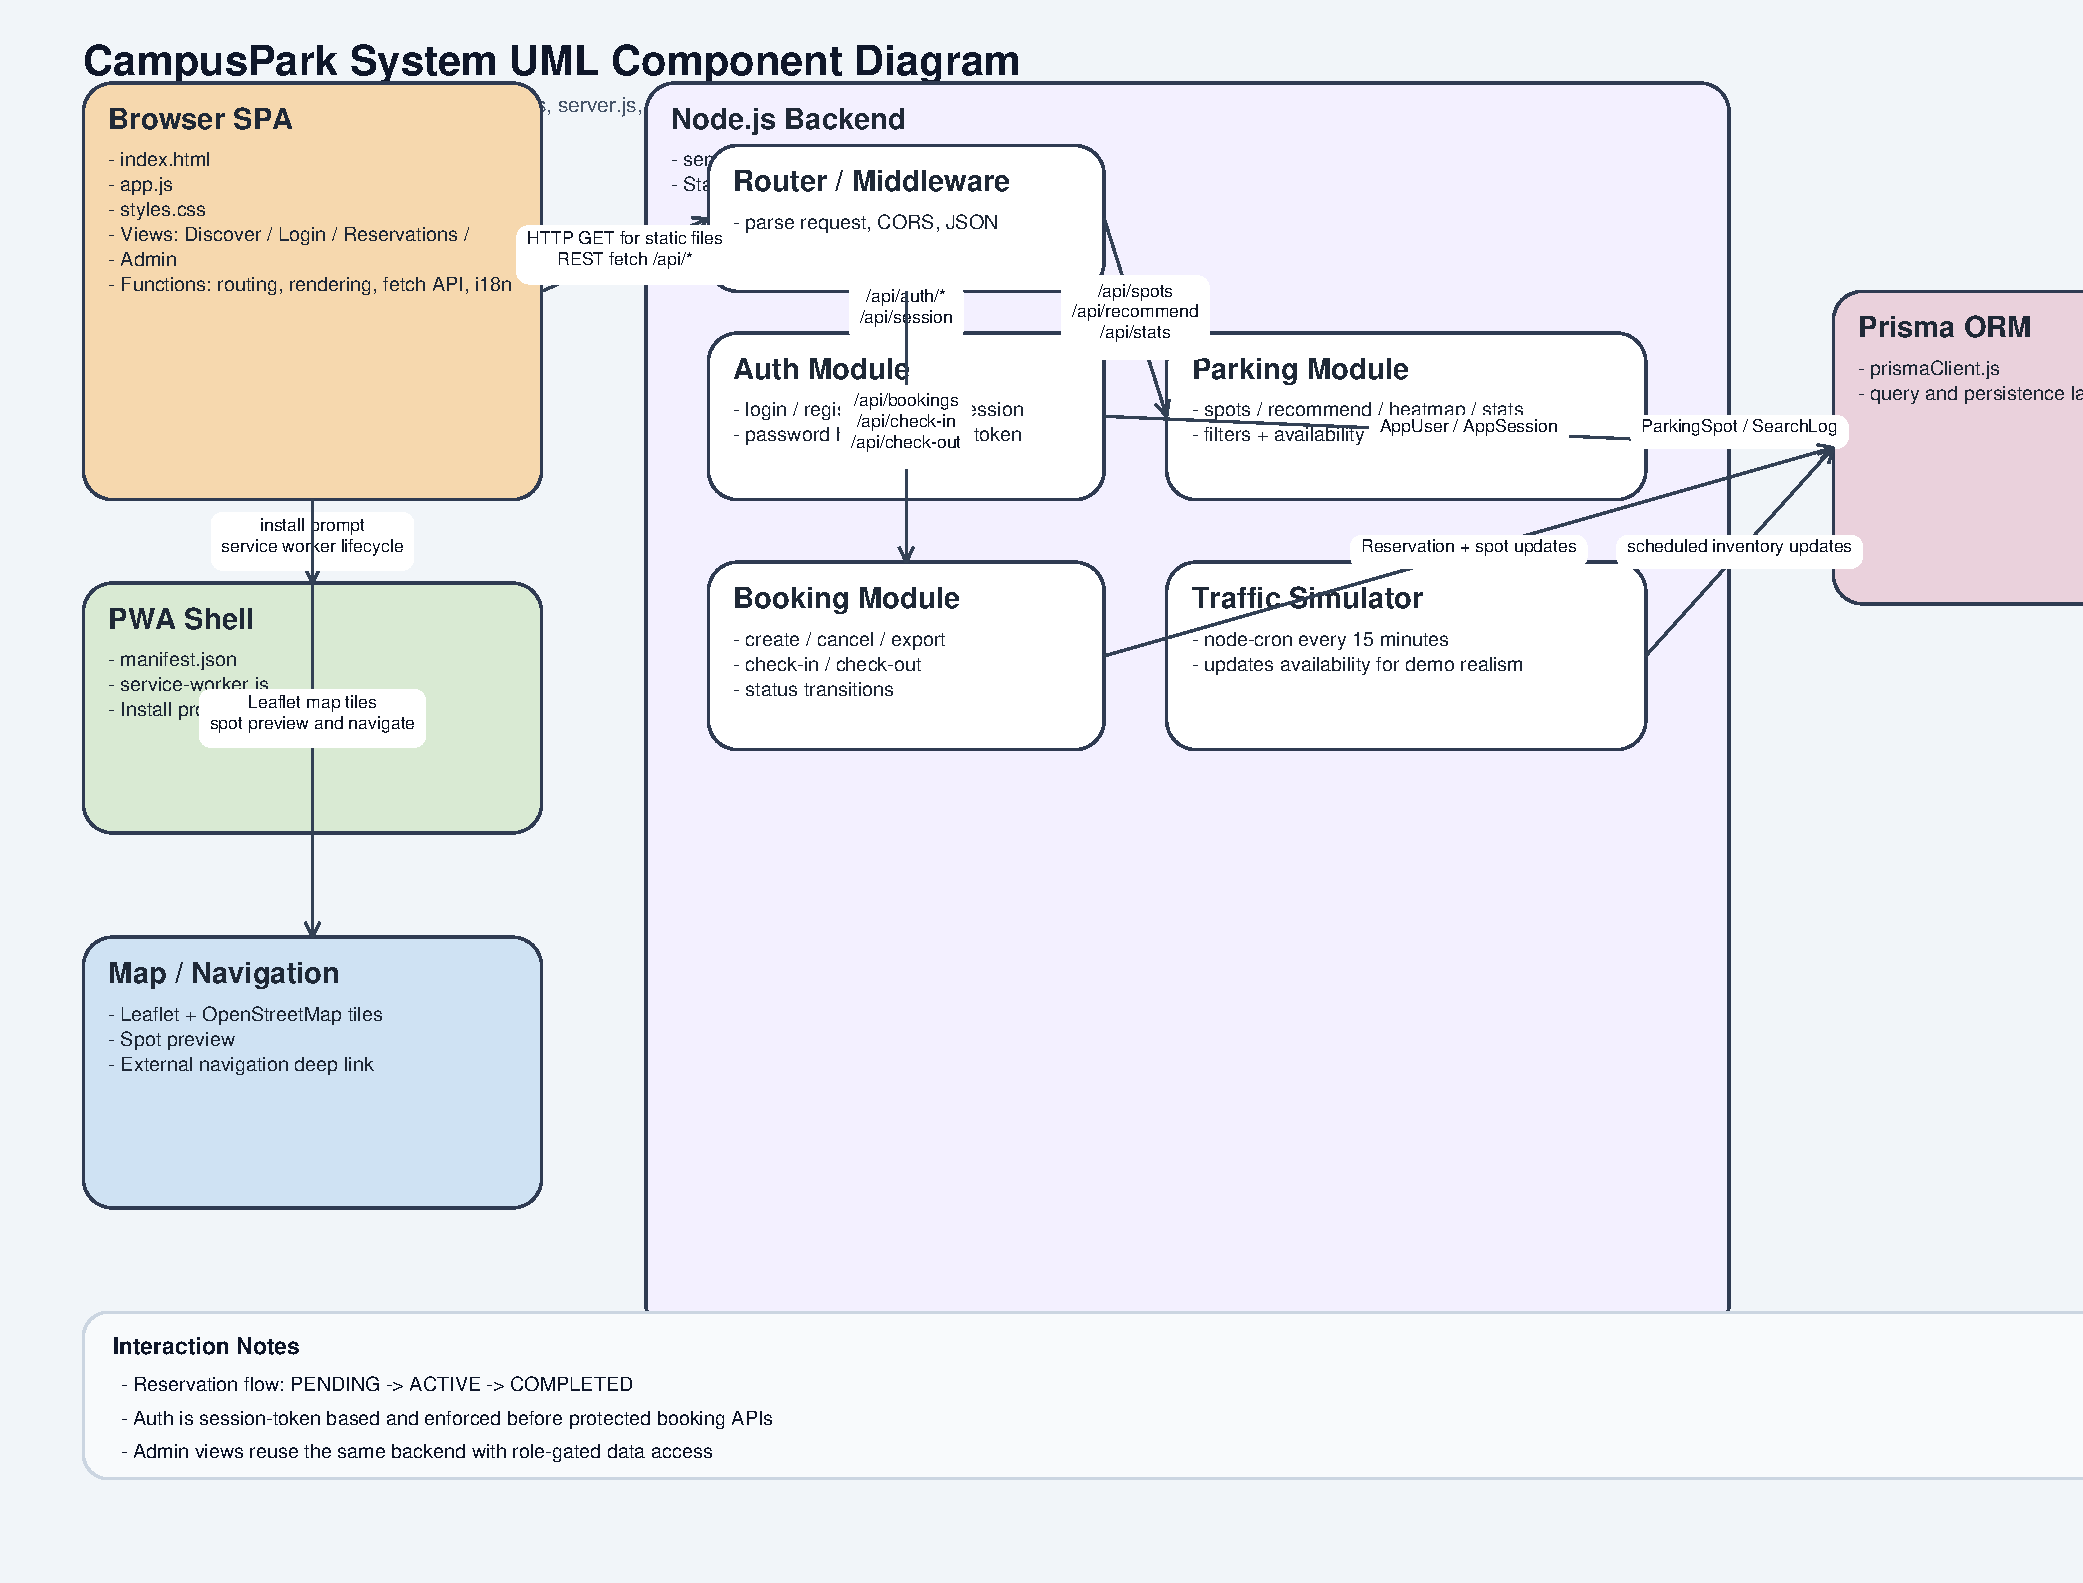
\includegraphics[width=\textwidth]{uml/campuspark-uml.pdf}
  \caption{CampusPark UML Component Diagram (Assignment 5).}
  \label{fig:uml}
\end{figure}

\subsection{Component Descriptions}

\textbf{Browser SPA} (\texttt{index.html}, \texttt{app.js}, \texttt{styles.css})
handles all page rendering, search filtering, map display, reservation flows,
and analytics event batching. There is no page reload between views -- routing
is done in JavaScript.

\textbf{PWA Shell} (\texttt{manifest.json}, \texttt{service-worker.js})
allows the app to be installed on a phone home screen and caches static assets
so the UI loads even on a slow connection.

\textbf{Map / Navigation} uses Leaflet with OpenStreetMap tiles for the
interactive map, Leaflet.heat for a demand heatmap, and OSRM for drawing
the driving route when a parking recommendation is shown.

\textbf{Node.js Backend} (\texttt{server.js}, around 2,000 lines) handles
all API requests, serves static files, manages sessions, enforces per-IP
rate limits, and runs a cron job for reservation expiry.

\textbf{Prisma ORM} handles database queries with a typed schema.
The six models are: \texttt{AppUser}, \texttt{AppSession}, \texttt{ParkingSpot},
\texttt{Reservation}, \texttt{FunnelEvent}, and \texttt{FeatureFlag}.

\textbf{PostgreSQL} stores all application data.
Availability counter updates use \texttt{LEAST()} in raw SQL to avoid
going above the physical capacity of a lot.

% ─────────────────────────────────────────────
\section{Core Features}

\subsection{Search and Reservation}
Users can filter by keyword, zone, arrival time, duration, and EV-only.
The Recommend button scores all spots on the server and highlights the
best match on the map. The booking form validates plate number and phone
format before submitting. Idempotency keys on the API prevent a double
booking if the user submits the form twice (e.g., due to a slow network).

\subsection{Route-Based Parking Assistant}
The departure input accepts a full address or a 5-digit ZIP code.
If the user enters a ZIP, the frontend appends the state and country
before sending it to the geocoder (e.g., \texttt{98006} becomes
\texttt{98006, WA, USA}). Address autocomplete shows Nominatim suggestions
with a 320\,ms debounce as the user types. Five ZIP chips are shown below
the input for common Seattle-area neighbourhoods.

\subsection{Analytics Dashboard}
The admin panel shows hourly booking counts and revenue by zone as Chart.js
bar charts, a 6-step user funnel (search through check-out) with conversion
rates, DAU/WAU/MAU counts, and a button to download all reservations as a
CSV file.

\subsection{Feature Flags}
Six feature flags are stored in the database and cached in memory for
30 seconds. Admins can toggle them in the dashboard without restarting
the server. Clients pick up the change within one TTL cycle.

\subsection{Other UX Details}
Dark mode is supported, using \texttt{prefers-color-scheme} for the
initial state and persisting the user's choice in localStorage.
Checked-in bookings display a QR code generated client-side from the
ticket code. A 5-step onboarding dialog appears once on first visit.
Active and pending reservations show a live countdown timer.

% ─────────────────────────────────────────────
\section{Algorithms}

\begin{description}[leftmargin=1.4em]
  \item[Dynamic pricing]
        The displayed price is \texttt{pricePerHour} $\times$ $D_h \times B_s$,
        where $D_h$ is a 24-point hourly demand multiplier (two peaks: 8\,AM and
        5\,PM on weekdays, scaled down 70\% on weekends) and $B_s$ is a
        deterministic per-spot offset in the range $[0.75,\,1.25]$ derived by
        hashing the spot name. EV spaces have a higher base \texttt{pricePerHour}
        set at seeding time rather than a runtime multiplier.

  \item[Surge pricing]
        When $\text{available}/\text{total} < 0.30$, the displayed price is
        multiplied by 1.5 and the original price is shown crossed out.

  \item[Recommendation scoring]
        $\text{score} = 0.5 \cdot s_{\text{prox}} + 0.3 \cdot s_{\text{avail}}
        + 0.2 \cdot s_{\text{crowd}}$,
        where $s_{\text{prox}}$ degrades linearly from 1 (on-route, $\leq$300\,m)
        to 0 (2\,km away), $s_{\text{avail}} = \min(\text{available}/10,\,1)$, and
        $s_{\text{crowd}} = 1 - D_h \times \text{popularityFactor}$ (lower current
        demand is better). Only spots with at least one free space are considered;
        the top-3 are returned.

  \item[Expiry cron]
        Every 60 seconds, \texttt{node-cron}~\cite{nodecron} selects all PENDING
        reservations created more than 5 minutes ago, marks them EXPIRED, and
        restores the lot's availability counter via
        \texttt{LEAST(availableSpots + 1, totalSpots)}.
\end{description}

% ─────────────────────────────────────────────
\section{Limitations}

\begin{enumerate}[leftmargin=1.4em]
  \item \textbf{Simulated occupancy.}
        The availability numbers come from a cron-based simulator, not from
        real gate sensors. The trends look realistic, but the counts do not
        match what is actually happening in any real lot.

  \item \textbf{Seattle only.}
        ZIP code normalisation hard-codes the state as Washington.
        Deploying this for a campus in another state would require changing
        that assumption.

  \item \textbf{No real payments.}
        The checkout flow calculates a fee and stores it, but there is no
        integration with a payment processor, so no money actually changes hands.

  \item \textbf{In-process rate limiting.}
        Rate limit counters live in the Node.js process memory. Running
        multiple server instances behind a load balancer would require
        moving them to a shared store like Redis.

  \item \textbf{Simple session model.}
        Sessions are random tokens stored in the database. There is no
        token expiry, refresh, or revocation beyond manually deleting the row.

  \item \textbf{No accessibility audit.}
        I have not tested the app with a screen reader or run an automated
        WCAG check. Some interactive elements may be hard to use with
        keyboard-only navigation.
\end{enumerate}

% ─────────────────────────────────────────────
\section{Future Work}

\begin{enumerate}[leftmargin=1.4em]
  \item Replace the simulator with actual gate/sensor data using a WebSocket
        connection, so the availability counts are real.

  \item Add a payment step using Stripe so users are actually charged at checkout,
        with refunds handled automatically on cancellation.

  \item Build a push notification flow so users get reminded before their
        parking window starts or when their booking is about to expire.

  \item Support multiple campuses by making the geographic region configurable
        rather than hard-coded to Seattle.

  \item Add a permit tier so students with annual permits can book from a
        separate reserved pool before the general inventory is opened.

  \item Do a proper accessibility pass -- fix focus order, add skip links,
        test with VoiceOver and NVDA, and check colour contrast ratios.

  \item Use the collected \texttt{FunnelEvent} and \texttt{SearchLog} data to
        train a simple demand forecasting model, which could help the system
        surface price or availability warnings before lots fill up.
\end{enumerate}

% ─────────────────────────────────────────────
\section{Conclusion}

CampusPark ended up covering more ground than I initially planned.
The core reservation workflow -- search, book, check in, check out --
works end to end, and the admin dashboard gives a decent view of what
is happening in the system. The main things I would improve with more
time are replacing the simulated data with real sources and adding
proper payment handling.

The source code is at
\href{https://github.com/sguanya-stack/campus-park}{github.com/sguanya-stack/campus-park}.

% ─────────────────────────────────────────────
\begin{thebibliography}{9}

\bibitem{nominatim}
OpenStreetMap contributors.
\textit{Nominatim}.
\url{https://nominatim.org/}, accessed April 2026.

\bibitem{osrm}
Project OSRM contributors.
\textit{Open Source Routing Machine}.
\url{https://project-osrm.org/}, accessed April 2026.

\bibitem{leaflet}
Agafonkin, V. et al.
\textit{Leaflet}.
\url{https://leafletjs.com/}, accessed April 2026.

\bibitem{prisma}
Prisma Data, Inc.
\textit{Prisma ORM}.
\url{https://www.prisma.io/docs/}, accessed April 2026.

\bibitem{nodecron}
Kelektiv.
\textit{node-cron}.
\url{https://github.com/kelektiv/node-cron}, accessed April 2026.

\bibitem{chartjs}
Chart.js contributors.
\textit{Chart.js}.
\url{https://www.chartjs.org/}, accessed April 2026.

\end{thebibliography}

\end{document}
